% Options for packages loaded elsewhere
\PassOptionsToPackage{unicode}{hyperref}
\PassOptionsToPackage{hyphens}{url}
\PassOptionsToPackage{dvipsnames,svgnames,x11names}{xcolor}
%
\documentclass[
  letterpaper,
  DIV=11,
  numbers=noendperiod]{scrartcl}

\usepackage{amsmath,amssymb}
\usepackage{iftex}
\ifPDFTeX
  \usepackage[T1]{fontenc}
  \usepackage[utf8]{inputenc}
  \usepackage{textcomp} % provide euro and other symbols
\else % if luatex or xetex
  \usepackage{unicode-math}
  \defaultfontfeatures{Scale=MatchLowercase}
  \defaultfontfeatures[\rmfamily]{Ligatures=TeX,Scale=1}
\fi
\usepackage{lmodern}
\ifPDFTeX\else  
    % xetex/luatex font selection
\fi
% Use upquote if available, for straight quotes in verbatim environments
\IfFileExists{upquote.sty}{\usepackage{upquote}}{}
\IfFileExists{microtype.sty}{% use microtype if available
  \usepackage[]{microtype}
  \UseMicrotypeSet[protrusion]{basicmath} % disable protrusion for tt fonts
}{}
\makeatletter
\@ifundefined{KOMAClassName}{% if non-KOMA class
  \IfFileExists{parskip.sty}{%
    \usepackage{parskip}
  }{% else
    \setlength{\parindent}{0pt}
    \setlength{\parskip}{6pt plus 2pt minus 1pt}}
}{% if KOMA class
  \KOMAoptions{parskip=half}}
\makeatother
\usepackage{xcolor}
\setlength{\emergencystretch}{3em} % prevent overfull lines
\setcounter{secnumdepth}{5}
% Make \paragraph and \subparagraph free-standing
\ifx\paragraph\undefined\else
  \let\oldparagraph\paragraph
  \renewcommand{\paragraph}[1]{\oldparagraph{#1}\mbox{}}
\fi
\ifx\subparagraph\undefined\else
  \let\oldsubparagraph\subparagraph
  \renewcommand{\subparagraph}[1]{\oldsubparagraph{#1}\mbox{}}
\fi


\providecommand{\tightlist}{%
  \setlength{\itemsep}{0pt}\setlength{\parskip}{0pt}}\usepackage{longtable,booktabs,array}
\usepackage{calc} % for calculating minipage widths
% Correct order of tables after \paragraph or \subparagraph
\usepackage{etoolbox}
\makeatletter
\patchcmd\longtable{\par}{\if@noskipsec\mbox{}\fi\par}{}{}
\makeatother
% Allow footnotes in longtable head/foot
\IfFileExists{footnotehyper.sty}{\usepackage{footnotehyper}}{\usepackage{footnote}}
\makesavenoteenv{longtable}
\usepackage{graphicx}
\makeatletter
\def\maxwidth{\ifdim\Gin@nat@width>\linewidth\linewidth\else\Gin@nat@width\fi}
\def\maxheight{\ifdim\Gin@nat@height>\textheight\textheight\else\Gin@nat@height\fi}
\makeatother
% Scale images if necessary, so that they will not overflow the page
% margins by default, and it is still possible to overwrite the defaults
% using explicit options in \includegraphics[width, height, ...]{}
\setkeys{Gin}{width=\maxwidth,height=\maxheight,keepaspectratio}
% Set default figure placement to htbp
\makeatletter
\def\fps@figure{htbp}
\makeatother
% definitions for citeproc citations
\NewDocumentCommand\citeproctext{}{}
\NewDocumentCommand\citeproc{mm}{%
  \begingroup\def\citeproctext{#2}\cite{#1}\endgroup}
\makeatletter
 % allow citations to break across lines
 \let\@cite@ofmt\@firstofone
 % avoid brackets around text for \cite:
 \def\@biblabel#1{}
 \def\@cite#1#2{{#1\if@tempswa , #2\fi}}
\makeatother
\newlength{\cslhangindent}
\setlength{\cslhangindent}{1.5em}
\newlength{\csllabelwidth}
\setlength{\csllabelwidth}{3em}
\newenvironment{CSLReferences}[2] % #1 hanging-indent, #2 entry-spacing
 {\begin{list}{}{%
  \setlength{\itemindent}{0pt}
  \setlength{\leftmargin}{0pt}
  \setlength{\parsep}{0pt}
  % turn on hanging indent if param 1 is 1
  \ifodd #1
   \setlength{\leftmargin}{\cslhangindent}
   \setlength{\itemindent}{-1\cslhangindent}
  \fi
  % set entry spacing
  \setlength{\itemsep}{#2\baselineskip}}}
 {\end{list}}
\usepackage{calc}
\newcommand{\CSLBlock}[1]{\hfill\break\parbox[t]{\linewidth}{\strut\ignorespaces#1\strut}}
\newcommand{\CSLLeftMargin}[1]{\parbox[t]{\csllabelwidth}{\strut#1\strut}}
\newcommand{\CSLRightInline}[1]{\parbox[t]{\linewidth - \csllabelwidth}{\strut#1\strut}}
\newcommand{\CSLIndent}[1]{\hspace{\cslhangindent}#1}

% load packages
\usepackage{geometry}
\usepackage{xcolor}
\usepackage{eso-pic}
\usepackage{fancyhdr}
\usepackage{sectsty}
\usepackage{fontspec}
\usepackage{titlesec}

%% Set page size with a wider right margin
\geometry{a4paper, total={170mm,257mm}, left=20mm, top=20mm, bottom=20mm, right=50mm}

%% Let's define some colours
\definecolor{uniblue}{HTML}{003865}
\definecolor{burgundy}{HTML}{7D2239}
\definecolor{cobalt}{HTML}{005C8A}
\definecolor{lavender}{HTML}{5B4D94}
\definecolor{leaf}{HTML}{006630}
\definecolor{moss}{HTML}{385A4F}
\definecolor{pillarbox}{HTML}{B30C00}
\definecolor{rust}{HTML}{9A3A06}
\definecolor{sandstone}{HTML}{52473B}
\definecolor{skyblue}{HTML}{005398}
\definecolor{slate}{HTML}{4F5961}
\definecolor{thistle}{HTML}{951272}

%\definecolor{light}{HTML}{E6E6FA} % original from template - redefined below as uni blue at 10 percent:
\colorlet{light}{uniblue!10}
%\definecolor{highlight}{HTML}{800080} % original from template - redefined below as uni's skyblue:
\colorlet{highlight}{skyblue}
%\definecolor{dark}{HTML}{330033} % original from template - redefined below as uni blue at 100 percent:
\colorlet{dark}{uniblue}

%% Let's add the border on the right hand side 
\AddToShipoutPicture{% 
    \AtPageLowerLeft{% 
        \put(\LenToUnit{\dimexpr\paperwidth-3cm},0){% 
            \color{light}\rule{3cm}{\LenToUnit\paperheight}%
          }%
     }%
     % logo
    \AtPageLowerLeft{% start the bar at the bottom right of the page
        \put(\LenToUnit{\dimexpr\paperwidth-2.25cm},27.2cm){% move it to the top right
            \color{light}\includegraphics[width=2.25cm]{_extensions/nrennie/PrettyPDF/uni_logo_boxed.jpg}
          }%
     }%
}

%% Style the page number
\fancypagestyle{mystyle}{
  \fancyhf{}
  \renewcommand\headrulewidth{0pt}
  \fancyfoot[R]{\thepage}
  \fancyfootoffset{3.5cm}
}
\setlength{\footskip}{20pt}

%% style the chapter/section fonts
\chapterfont{\color{uniblue}\fontsize{20}{16.8}\selectfont}
\sectionfont{\color{uniblue}\fontsize{20}{16.8}\selectfont}
\subsectionfont{\color{skyblue}\fontsize{14}{16.8}\selectfont}
\titleformat{\subsection}
  {\color{uniblue!90}\sffamily\Large\bfseries}{\thesubsection}{1em}{}[{\titlerule[0.8pt]}]
\subsubsectionfont{\color{cobalt}}

\renewcommand\thesection{\color{slate}\arabic{section}}
  
% left align title
\makeatletter
\renewcommand{\maketitle}{\bgroup\setlength{\parindent}{0pt}
\begin{flushleft}
  {\color{uniblue}\sffamily\huge\textbf{\@title}} \vspace{0.3cm} \newline
  {\Large {\@subtitle}} \newline
  \@author
\end{flushleft}\egroup
}
\makeatother

%% Use some custom fonts
\setsansfont{Ubuntu}[
    Path=_extensions/nrennie/PrettyPDF/Ubuntu/,
    Scale=0.9,
    Extension = .ttf,
    UprightFont=*-Regular,
    BoldFont=*-Bold,
    ItalicFont=*-Italic,
    ]

\setmainfont{Ubuntu}[
    Path=_extensions/nrennie/PrettyPDF/Ubuntu/,
    Scale=0.9,
    Extension = .ttf,
    UprightFont=*-Regular,
    BoldFont=*-Bold,
    ItalicFont=*-Italic,
    ]
\KOMAoption{captions}{tableheading}
\makeatletter
\@ifpackageloaded{tcolorbox}{}{\usepackage[skins,breakable]{tcolorbox}}
\@ifpackageloaded{fontawesome5}{}{\usepackage{fontawesome5}}
\definecolor{quarto-callout-color}{HTML}{909090}
\definecolor{quarto-callout-note-color}{HTML}{0758E5}
\definecolor{quarto-callout-important-color}{HTML}{CC1914}
\definecolor{quarto-callout-warning-color}{HTML}{EB9113}
\definecolor{quarto-callout-tip-color}{HTML}{00A047}
\definecolor{quarto-callout-caution-color}{HTML}{FC5300}
\definecolor{quarto-callout-color-frame}{HTML}{acacac}
\definecolor{quarto-callout-note-color-frame}{HTML}{4582ec}
\definecolor{quarto-callout-important-color-frame}{HTML}{d9534f}
\definecolor{quarto-callout-warning-color-frame}{HTML}{f0ad4e}
\definecolor{quarto-callout-tip-color-frame}{HTML}{02b875}
\definecolor{quarto-callout-caution-color-frame}{HTML}{fd7e14}
\makeatother
\makeatletter
\@ifpackageloaded{caption}{}{\usepackage{caption}}
\AtBeginDocument{%
\ifdefined\contentsname
  \renewcommand*\contentsname{Table of contents}
\else
  \newcommand\contentsname{Table of contents}
\fi
\ifdefined\listfigurename
  \renewcommand*\listfigurename{List of Figures}
\else
  \newcommand\listfigurename{List of Figures}
\fi
\ifdefined\listtablename
  \renewcommand*\listtablename{List of Tables}
\else
  \newcommand\listtablename{List of Tables}
\fi
\ifdefined\figurename
  \renewcommand*\figurename{Figure}
\else
  \newcommand\figurename{Figure}
\fi
\ifdefined\tablename
  \renewcommand*\tablename{Table}
\else
  \newcommand\tablename{Table}
\fi
}
\@ifpackageloaded{float}{}{\usepackage{float}}
\floatstyle{ruled}
\@ifundefined{c@chapter}{\newfloat{codelisting}{h}{lop}}{\newfloat{codelisting}{h}{lop}[chapter]}
\floatname{codelisting}{Listing}
\newcommand*\listoflistings{\listof{codelisting}{List of Listings}}
\makeatother
\makeatletter
\makeatother
\makeatletter
\@ifpackageloaded{caption}{}{\usepackage{caption}}
\@ifpackageloaded{subcaption}{}{\usepackage{subcaption}}
\makeatother
\makeatletter
\@ifpackageloaded{tcolorbox}{}{\usepackage[skins,breakable]{tcolorbox}}
\makeatother
\makeatletter
\@ifundefined{shadecolor}{\definecolor{shadecolor}{rgb}{.97, .97, .97}}{}
\makeatother
\makeatletter
\@ifundefined{codebgcolor}{\definecolor{codebgcolor}{named}{light}}{}
\makeatother
\makeatletter
\ifdefined\Shaded\renewenvironment{Shaded}{\begin{tcolorbox}[boxrule=0pt, breakable, colback={codebgcolor}, enhanced, sharp corners, frame hidden]}{\end{tcolorbox}}\fi
\makeatother
\ifLuaTeX
  \usepackage{selnolig}  % disable illegal ligatures
\fi
\usepackage{bookmark}

\IfFileExists{xurl.sty}{\usepackage{xurl}}{} % add URL line breaks if available
\urlstyle{same} % disable monospaced font for URLs
\hypersetup{
  pdftitle={Sampling and Monitoring Networks},
  colorlinks=true,
  linkcolor={highlight},
  filecolor={Maroon},
  citecolor={Blue},
  urlcolor={highlight},
  pdfcreator={LaTeX via pandoc}}

\title{Sampling and Monitoring Networks}
\author{}
\date{}

\begin{document}
\maketitle

\pagestyle{mystyle}

\section{Overview}\label{overview}

This session will focus on how environmental and ecological data are
obtained, specifically through sampling. Sampling is a fundamental
concept in data analysis, especially in environmental data.

We use samples in environmental data in situations where it is not
possible to measure the entire population. In environmental settings,
this could be because:

\begin{itemize}
\tightlist
\item
  The population is too large.
\item
  Some or all of the population is difficult, expensive, or even
  impossible to reach.
\item
  The samples may be \emph{destructive}, i.e., taking the sample causes
  permanent damage to the object being measured.
\end{itemize}

We want to use the information we obtain on the \textbf{sample} in order
to make \emph{inference} on the \textbf{population}.

\begin{center}
\includegraphics[width=5.38542in,height=\textheight]{images/sample2pop.png}
\end{center}

\section{Designing an ecological/environmental
study}\label{designing-an-ecologicalenvironmental-study}

When we design an environmental or an ecological study we should focud
on these steps:

\begin{enumerate}
\def\labelenumi{\arabic{enumi}.}
\item
  Define the study objectives.
\item
  Summarize the environmental context.
\item
  Identify the target population.
\item
  Select an appropriate sampling design.
\item
  Implement and summarize.
\end{enumerate}

\subsection*{Step 1 --- Define the study
objectives}\label{step-1-define-the-study-objectives}
\addcontentsline{toc}{subsection}{Step 1 --- Define the study
objectives}

We need to define clear and simple objectives for our study. What is the
key question or hypothesis?These will be driven by the properties of our
data that we would like to measure:

\begin{itemize}
\tightlist
\item
  Characteristics of a variable, e.g.~mean, median, variance.
\item
  Temporal or spatial trends of a variable.
\item
  Frequency of events, e.g.~number of pollution events, species
  abundance or occurrence.
\end{itemize}

\begin{tcolorbox}[enhanced jigsaw, arc=.35mm, colframe=quarto-callout-note-color-frame, breakable, colback=white, opacityback=0, colbacktitle=quarto-callout-note-color!10!white, toptitle=1mm, toprule=.15mm, coltitle=black, title=\textcolor{quarto-callout-note-color}{\faInfo}\hspace{0.5em}{Example: water quality}, left=2mm, rightrule=.15mm, bottomrule=.15mm, titlerule=0mm, bottomtitle=1mm, opacitybacktitle=0.6, leftrule=.75mm]

What is the spatial or temporal variability of water quality across a
River Surveillance Network (RSN)?

\begin{figure}[H]

{\centering \includegraphics[width=3.95833in,height=\textheight]{images/EA_OS1.jpg}

}

\caption{OS Open Rivers network represented in blue lines and the pink
dots representing the Environment Agency monitoring stations.}

\end{figure}%

\end{tcolorbox}

\subsection*{Step 2 --- Consider the
context}\label{step-2-consider-the-context}
\addcontentsline{toc}{subsection}{Step 2 --- Consider the context}

We have to think about the context of the question we are asking. This
means understanding the nature of our data, which is essential to
ensuring we have a \textbf{representative} sample.

For example, if we're measuring a river, we need to know about the
depth, width, and current. If we are sampling in a forest we need to
know about vegetation and wildlife.

\subsection*{Step 3 --- Identify the target
population}\label{step-3-identify-the-target-population}
\addcontentsline{toc}{subsection}{Step 3 --- Identify the target
population}

The population is the set of all possible objects that could be sampled.

\begin{itemize}
\tightlist
\item
  All the fish in a lake.
\item
  All oak trees over 5m tall in a particular part of a forest.
\item
  Every river within a particular water network.
\end{itemize}

Sometimes the population is actually what we are trying to measure,
e.g.~``How many red squirrels live in the Cairngorms National Park?''

\begin{tcolorbox}[enhanced jigsaw, arc=.35mm, colframe=quarto-callout-note-color-frame, breakable, colback=white, opacityback=0, colbacktitle=quarto-callout-note-color!10!white, toptitle=1mm, toprule=.15mm, coltitle=black, title=\textcolor{quarto-callout-note-color}{\faInfo}\hspace{0.5em}{Example: Water quality}, left=2mm, rightrule=.15mm, bottomrule=.15mm, titlerule=0mm, bottomtitle=1mm, opacitybacktitle=0.6, leftrule=.75mm]

\textbf{Target population}:
\href{https://www.arcgis.com/home/item.html?id=a0a065da1ab642e69bd1a5e018b4ddf4}{RSN}
1:250k with over 1.4 million reaches (a discrete segment of a river with
relatively uniform characteristics) .

\textbf{Characterise environmental conditions} of the target population
such as Water Quality Indicators, i.e., we need to define our
\textbf{response variable}:

\begin{itemize}
\item
  Macroinvertebrates composition obtained from the
  \href{https://environment.data.gov.uk/dataset/8d1422b3-c960-4ed9-a324-40eefb0c016e}{RICT
  Model 44} network (1:50k scale and trimmed to match the RSN network).
  E.g., \textbf{WHPT-ASPT} (\emph{Walley Hawkes Paisley Trigg Average
  Score Per Taxon}) is a~\textbf{biological metric}~used to evaluate the
  ecological health of rivers based on the presence and sensitivity
  of~macroinvertebrate~(e.g., insects, worms, snails) communities.~
\item
  Orthophosphate \([\text{PO}_4]^{3-}\) concentrations (mg/L)
\end{itemize}

\end{tcolorbox}

\subsection*{Step 4 --- Select a sampling
design}\label{step-4-select-a-sampling-design}
\addcontentsline{toc}{subsection}{Step 4 --- Select a sampling design}

There are a number of sampling designs which are commonly used for
environmental data:

\begin{itemize}
\tightlist
\item
  Simple random sampling.
\item
  Stratified random sampling.
\item
  Systematic sampling.
\item
  Spatial sampling.
\end{itemize}

We will discuss some of these in more detail during the course.

\subsection*{Step 5 --- Implement and
summarise}\label{step-5-implement-and-summarise}
\addcontentsline{toc}{subsection}{Step 5 --- Implement and summarise}

\begin{itemize}
\item
  \textbf{Data collection} - what information is being collected and
  how? E.g., biological elements, river habitat surveys,
  physico-chemical elements, toxic chemicals, invasive non-native
  species, physical properties, etc. What technical equipment or
  techniques are used to measure these elements?
\item
  \textbf{Implementation} - deploying the network and measuring the
  quantities of interest. Be aware of practical challenges that might
  impact the subsequent analysis such as: accessibility contains to the
  selected sampling site, landowner permission, safety issues,
  unfavorable environmental conditions, etc.
\end{itemize}

Often statisticians will not actually carry out the sampling, but will
instead rely on field experts in many cases. Once we receive the data,
it's important to assess the data for censoring, outliers, missingness.
We can then fit an appropriate statistical model. Finally, we should
report our results in clear language, including uncertainty where
appropriate.

In this session we will look at different sampling schemes commonly used
in environmental and ecological monitoring. A sampling strategy
integrates both sample selection methods from a target population and
estimation techniques to infer population attributes from sample
measurements.

Such attributes can be viewed as a quantitative combination of
population values such as the mean Orthophosphate \([\text{PO}_4]^{3-}\)
concentration or the total number of macroinvertebrates in a river.
Likewise, an \emph{estimator} is a mathematical expression or a function
of the sample that provide us with a \emph{estimate} of the population
parameter. For instance, let \(\theta\) denote the population parameter
of interest (e.g., the population mean), then \(\hat{\theta}\)
represents its estimator (see {[}additional notes{]}\{about.qmd\} on
estimator properties). Typically, the value of \(\theta\) is unknown and
it is unfeasible to measure all \(N\) elements of the population. Thus,
we select and measure \(n < N\) units to estimate \(\theta\). The
question now is how do we select such units?

\section{Sampling Methods}\label{sampling-methods}

\subsection{Simple Random Sampling}\label{simple-random-sampling}

As the name suggests, this is the simplest form of sampling. Every
object in our population has an \textbf{equal probability} of being
included in the sample. This requires us to have a complete list of the
population members, or a sampling frame covering the entire region. We
then generate a set of \(n\) random digits which identify the
individuals or objects to be included in a study.

For a sample of size \(n\), denoted \(y_1, \ldots, y_n\), we can compute
the sample mean as \[\bar{y} = \frac{\sum_{i=1}^n y_i}{n}.\]

We can then compute the estimated population variance as
\[s^2 =\frac{\sum_{i=1}^n (y_i - \bar{y})^2}{n-1}.\]

As well as estimating the population mean and variance, we also have to
think about the uncertainty surrounding these estimates. This is what a
confidence interval is typically representing.

Our sample of size \(n\) is just one of many possible samples of size
\(n\) which we could have obtained. We must take this into account when
considering the uncertainty associated with our sample mean. This is
known as \textbf{sampling variability}. We can compute this as:
\[Var({\bar{y}}) = \frac{s^2}{n}\left(1 - \frac{n}{N}\right).\] Here,
\((1 - \frac{n}{N})\) is what is known as a \textbf{finite population
correction} (FPC), which accounts for the proportion of the data that
remains unknown.

\begin{tcolorbox}[enhanced jigsaw, arc=.35mm, colframe=quarto-callout-important-color-frame, breakable, colback=white, opacityback=0, colbacktitle=quarto-callout-important-color!10!white, toptitle=1mm, toprule=.15mm, coltitle=black, title={Task 1}, left=2mm, rightrule=.15mm, bottomrule=.15mm, titlerule=0mm, bottomtitle=1mm, opacitybacktitle=0.6, leftrule=.75mm]

To monitor patterns of weekly water consumption, a town conducted a SRS
of \(n=100\) homes. The town records showed that there were \(N=5392\)
residential dwellings with water meter in town. Water consumption was
recorded in 100-gallon units. The sample average consumption was
\(\bar{y} = 12.5\) 100-gallons units per week and the sample variance
was \(s^2 = 1352\) (100-gallon units)\(^2\). The local authority is
interested in estimating the town's total weekly residential water
usage. An unbiased estimator of a population total under SRS was given
by Horvitz-Thompson (1963) as:

\begin{equation}\phantomsection\label{eq-HT}{
\hat{\tau} = N\bar{y}
}\end{equation}

Using HT estimator, calculate the town's total weekly residential water
consumption. Then. derive the variance of this estimator and compute the
standard deviation (square-root of the variance) for the town's totals.

See Solution

Using Equation~\ref{eq-HT}, the estimated weekly residential water use
town totals is \(5392 \times 12.5 = 67 400\) 100-gallon units. Then, the
variance and standard deviation of \(\hat{\tau}\) are :

\[
\begin{aligned}
Var(\hat{\tau}) &= Var(N\bar{y}) \\
&= N^2 Var(\bar{y}) \\
&= N^2 \times\dfrac{s^2}{n} \left(1- \dfrac{n}{N}\right)\\
&= 5392^2 \times \frac{1352}{100} \left(1- \frac{100}{5392}\right)\\
&\Rightarrow\\
\sqrt{Var(\tau)} &=  5392 \times \sqrt{\frac{1352}{100} \left(1- \frac{100}{5392}\right)} \\
&= 19,641~ \text{ 100-gallon units.}
\end{aligned}
\]

\end{tcolorbox}

\subsection{Stratified Sampling}\label{stratified-sampling}

\begin{tcolorbox}[enhanced jigsaw, arc=.35mm, colframe=quarto-callout-note-color-frame, breakable, colback=white, opacityback=0, colbacktitle=quarto-callout-note-color!10!white, toptitle=1mm, toprule=.15mm, coltitle=black, title={Example: Cobalt-60 in sediment}, left=2mm, rightrule=.15mm, bottomrule=.15mm, titlerule=0mm, bottomtitle=1mm, opacitybacktitle=0.6, leftrule=.75mm]

Cobalt-60 is a synthetic radioactive isotope of cobalt produced in
nuclear reactors. We may be interested in estimating how much of this is
in the sediment of a river estuary. This map is colour coded by
different sediment types. How might we make use of this information when
sampling?

\begin{center}
\includegraphics[width=5.20833in,height=\textheight]{images/Cobalt.png}
\end{center}

\end{tcolorbox}

Stratified sampling involves dividing the population into two or more
groups (or strata) which have something in common. Divide the dataset of
size \(N\) into \(L\) non-overlapping strata such that within-strata
variability is less than between-strata variability. We then ensure that
each of our strata are represented in our sample, and take this into
account in our final estimates.

We ensure that each of these strata are represented proportionally
within our sample (known as \textbf{proportional allocation}). Samples
are still taken randomly within each stratum.

\begin{tcolorbox}[enhanced jigsaw, arc=.35mm, colframe=quarto-callout-note-color-frame, breakable, colback=white, opacityback=0, colbacktitle=quarto-callout-note-color!10!white, toptitle=1mm, toprule=.15mm, coltitle=black, title={Example: Cobalt-60 in sediment (continued)}, left=2mm, rightrule=.15mm, bottomrule=.15mm, titlerule=0mm, bottomtitle=1mm, opacitybacktitle=0.6, leftrule=.75mm]

The map below shows black dots at the sampling locations that were
chosen using stratified sampling. There are 50 sampling locations in
total, and we can see that these are found proportionally across the
strata. E.g., there are very few sampling locations within the light
yellow region, reflecting that region's smaller area. Stratified
sampling has ensured that we do, however, have at least some sampling
locations within each strata.

\begin{center}
\includegraphics[width=5.20833in,height=\textheight]{images/Cobalt2.png}
\end{center}

\end{tcolorbox}

Let \(N_1, \ldots, N_L\) be the populations of our \(L\) strata, and
\(n_1, \ldots, n_L\) be the number of samples taken from each. It is
straightforward to obtain sample means \(y_1, \ldots, y_L\) and sample
variances \(s_1^2, \ldots, s_L^2\) for each stratum.

Then we compute the overall sample mean as
\[\bar{y} = \frac{\sum_{l=1}^L \left( N_l y_l \right)}{N}.\]

We can also compute the variance of the sample mean as
\[Var(\bar{y}) = \sum_{l=1}^L \left[ \left(\frac{N_l}{N}\right)^2 \frac{s_l^2}{n_l} \left(1 - \frac{n_l}{N_l} \right) \right].\]

\subsection{Systematic Sampling}\label{systematic-sampling}

Systematic sampling is a sampling method which makes use of a natural
ordering that exists in data. We wish to take a sample of size \(n\)
from a population of size \(N\), which means every \(k = \frac{N}{n}\)
objects are sampled. For systematic sampling, we select our first unit
at random, then select every \(k\)th unit in a systematic way.

For example, if we have \(N=50\) and \(n=5\), then \(k=10\). If our
first unit is 2, our sample becomes units 2, 12, 22, 32, 42.

\textbf{Advantages}

\begin{itemize}
\tightlist
\item
  Convenient and quick.
\item
  Well spaced across the study.
\item
  Sort of random --- every object has an equal chance of selection.
\end{itemize}

\textbf{Disadvantages}

\begin{itemize}
\tightlist
\item
  May not be representative.
\item
  Systematic patterns in the data can be overlooked.
\item
  Extremely deterministic --- estimation of variance particularly
  difficult.
\end{itemize}

\subsection{Spatial Sampling}\label{spatial-sampling}

Spatial sampling is required when our data have an attribute that is
spatially continuous. For example, if we are measuring water quality in
a lake, we may have a three-dimensional coordinate system of
\emph{length}, \emph{width} and \emph{depth}. In some cases, it is
possible to measure at any one of these locations, and simple random
sampling or stratified sampling can be used. There are many examples
where it is not possible or convenient to do so, in which case some form
of systematic sampling may be used.

Spatial sampling often uses a systematic sampling scheme based on
\textbf{transects}. A transect is a straight line along which samples
are taken. The starting point, geographical orientation and number of
samples are chosen as part of the sampling scheme. Samples will then be
either taken at random points along the length of the line
(\emph{continuous sampling}) or systematically placed points
(\emph{systematic sampling}).

Suppose we need to take samples of water quality on a lake. Our sampling
scheme may use multiple transects simultaneously.

\begin{center}
\includegraphics[width=5.20833in,height=\textheight]{images/Transect.png}
\end{center}

\subsubsection{\texorpdfstring{\textbf{Distance
sampling}}{Distance sampling}}\label{distance-sampling}

In ecology, \emph{distance sampling,} is a widely used spatial sampling
method for estimating animal abundance or population density by
measuring the perpendicular distances from a transect line or point to
detected individuals \textbf{?@fig-dist\_sampling} . The methods assumes
that the probability of observing animals decreases with increasing
distance from the observer according to a specific detection function.
The distance data are modelled using this detection function to account
for imperfect detection and estimate the proportion of missed
individuals in the study area.

\subsubsection{\texorpdfstring{\textbf{Quadrats}}{Quadrats}}\label{quadrats}

In some cases, we will instead be interested in trying to understand the
frequency of a certain species across space. A \textbf{quadrat} is a
tool used in ecology and other settings for this purpose. A series of
squares (quadrats) of a fixed size are placed in the habitat of
interest, and the species within the quadrats are counted. The number of
quadrats, and their positions and orientations are chosen as part of the
sampling scheme.

\begin{center}
\includegraphics[width=5.20833in,height=\textheight]{images/Quadrat.png}
\end{center}

\subsubsection{Grid Sampling}\label{grid-sampling}

It may often be useful to use a regular grid to make sampling convenient
and efficient. The grid is overlaid on the spatial region, and a fixed
number of samples (usually one) is taken from each grids square. We
choose the size of the grid such that the number of squares relates to
the number of samples we require. For example, for a region of size 5km
\(\times\) 5km, choosing 1km \(\times\) 1km grid squares would give us
25 squares in total.

There are a few different types of grid sampling.

\begin{itemize}
\tightlist
\item
  \textbf{Aligned Grid} --- we take a sample from the \emph{same}
  (randomly selected) coordinates within each square.
\item
  \textbf{Centrally Aligned Grid} --- we take a sample from the
  \emph{central} coordinates of each square.
\item
  \textbf{Unaligned Grid} --- each grid square has a sample taken from
  \emph{different} randomly selected coordinates.
\item
  \textbf{Triangular Grid} --- this is a modified version of the aligned
  grid where the points are fixed based on a triangular arrangement.
\end{itemize}

\begin{center}
\includegraphics[width=5.20833in,height=\textheight]{images/Grids.jpg}
\end{center}

The aligned and centrally aligned grids are convenient but may miss
systematic patterns in the data. The unaligned grid avoids this, and
combines the advantages of simple random sampling and stratified
sampling. However, it can be inefficient for collection. The triangular
grid can perform well in specific cases where the spatial correlation
structures varies with direction.

\begin{tcolorbox}[enhanced jigsaw, arc=.35mm, colframe=quarto-callout-tip-color-frame, breakable, colback=white, opacityback=0, colbacktitle=quarto-callout-tip-color!10!white, toptitle=1mm, toprule=.15mm, coltitle=black, title={Exercise 1: Heights of trees}, left=2mm, rightrule=.15mm, bottomrule=.15mm, titlerule=0mm, bottomtitle=1mm, opacitybacktitle=0.6, leftrule=.75mm]

Aim: Estimate the average height of trees which are uniformly
distributed within a 10 km\(^2\) forest.

\begin{center}
\includegraphics[width=4.25in,height=\textheight]{images/Trees.jpg}
\end{center}

\begin{itemize}
\tightlist
\item
  What is the population here?
\end{itemize}

Solution

The \textbf{population} is all trees in the forest.

\begin{itemize}
\tightlist
\item
  What are the sampling units?
\end{itemize}

Solution

Our \textbf{sampling units} are individual trees.

\begin{itemize}
\tightlist
\item
  What type of sampling scheme would be appropriate here?
\end{itemize}

Solution

Simple random sampling would likely be appropriate here, since it allows
us to cover the large area of the forest at low ``cost'' (time and
financial). The trees are uniformly distributed across the forest, so no
need for strata. You could argue for systematic sampling using a grid or
quadrats, but this may make analysis more complex.

\end{tcolorbox}

\begin{tcolorbox}[enhanced jigsaw, arc=.35mm, colframe=quarto-callout-tip-color-frame, breakable, colback=white, opacityback=0, colbacktitle=quarto-callout-tip-color!10!white, toptitle=1mm, toprule=.15mm, coltitle=black, title={Exercise 2: Chlorophyll-a in Lake Balaton}, left=2mm, rightrule=.15mm, bottomrule=.15mm, titlerule=0mm, bottomtitle=1mm, opacitybacktitle=0.6, leftrule=.75mm]

Aim: Estimate the average level of chlorophyll-a on Lake Balaton,
Hungary. Levels are heavily affected by differences in the levels of
nutrients along the length of the lake (known as a `trophic gradient').

\begin{center}
\includegraphics[width=4.32292in,height=\textheight]{images/Balaton.png}
\end{center}

\begin{itemize}
\tightlist
\item
  What is the population here?
\end{itemize}

Solution

The \textbf{population} is all possible water samples from the lake.

\begin{itemize}
\tightlist
\item
  What are the sampling units?
\end{itemize}

Solution

Our \textbf{sampling units} are individual water samples.

\begin{itemize}
\tightlist
\item
  What type of sampling scheme would be appropriate here?
\end{itemize}

Solution

Stratified random sampling seems appropriate here due to
\emph{heterogeneity} in the lake. We could design transects which cover
most regions of the lake. However, may be difficulty accessing all areas
by boat. Also, there are potential issues with the boat itself
disrupting the levels.

\end{tcolorbox}

\section{Sample Size}\label{sample-size}

A crucial part of sampling is identifying the appropriate sample size
for our study. If the sample is \emph{too small}, it will not be
sufficiently representative of the population. If the sample is
\emph{too big}, it will be expensive and time consuming to collect,
which may defeat the purpose of using sampling in the first place.

It is therefore important that we understand exactly what it is that we
want from our sampling process. We can think about it in terms of two
key aspects, \textbf{power} and \textbf{precision}.

\begin{itemize}
\tightlist
\item
  Precision --- how accurately do I want (or need) to estimate the mean,
  median, variance etc?
\item
  Power --- how small a difference is it important to detect, and with
  what degree of certainty?
\end{itemize}

We can use the formula for the confidence interval to help compute
sample sizes.

The general form of a 95\% confidence interval for the population mean,
\(\mu\), is \[\bar{x} \pm t_{1-\alpha/2} \sqrt{Var({\bar{x})}}\]

The width of the interval is determined by the estimated standard error,
\(\sqrt{Var({\bar{x})}}\), and we know the formula for this contains
\(n\). Therefore, if we know how wide we need our interval to be
(i.e.~the precision), we can calculate the \(n\) required to do that.

Let our maximum required standard error be denoted as \(U\). Then we
know:

\begin{itemize}
\tightlist
\item
  \(\sqrt{Var({\bar{x})}} \leq U\)
\item
  \(\frac{\sqrt{s^2}}{\sqrt{n}} \leq U\)
\item
  \(\sqrt{n} \geq \frac{\sqrt{s^2}}{U}\)
\end{itemize}

Here, \(s^2\) is the \textbf{sample} variance. This calculation requires
us to use \(s^2\), the variance of our sample. But we don't have the
sample yet --- the whole point of this exercise is to determine the size
of our sample. So what can we use instead? Typically we will use
knowledge from prior studies where available, or will commission a small
pilot study.

\begin{tcolorbox}[enhanced jigsaw, arc=.35mm, colframe=quarto-callout-tip-color-frame, breakable, colback=white, opacityback=0, colbacktitle=quarto-callout-tip-color!10!white, toptitle=1mm, toprule=.15mm, coltitle=black, title={Exercise 3: PCB in salmon}, left=2mm, rightrule=.15mm, bottomrule=.15mm, titlerule=0mm, bottomtitle=1mm, opacitybacktitle=0.6, leftrule=.75mm]

Polychlorinated biphenyl (PCB) is a carcinogenic pollutant often found
in fish. We wish to estimate the mean PCB level in the salmon in a fish
farm, and require a precision level (estimated standard error) of
\(\pm 0.1 \mbox{mg/kg}^2\). We know from previous studies that the
variation of PCB in salmon flesh is \(3.19^2\). How large a sample do we
need?

\emph{Answer (as an integer):} \_\_\_\_

Solution

We can solve our prior equation as
\[n \geq \left(\frac{s}{u} \right)^2 = \left(\frac{3.19}{0.1} \right)^2 = 1018.\]

We have estimated that we need a minimum sample size of 1018 to obtain
the required precision.

\end{tcolorbox}

In Exercise 3 above, we calculated the minimum sample size required to
obtain a required precision. In some cases this may be impractical, in
which case we may have to settle for a lower precision.

\subsection{Sample Size in Stratified
sampling}\label{sample-size-in-stratified-sampling}

For stratified sampling, this process is much more complicated. As well
as considering the sample size, we also have to think about how to
allocate our samples across the strata. A common approach is to specify
a \textbf{cost model}, where we take into account the different costs of
sampling each stratum. The aim is to minimize the estimated standard
error for a given total cost.

Let \(C\) be the overall cost, let \(c_0\) be the fixed overhead costs
of the survey and let \(c_l\) be the cost per sample in stratum \(l\).
Then our cost model is \[C = c_0 + \sum_{l=1}^L c_l n_l\]

Typically \(C\) is fixed, and the goal is to select the values of
\(n_l\) which allow us to obtain the best possible estimate.

Now let \(\omega_l = N_l/N\) be the proportion of the overall population
which is found within stratum \(l\). Also let \(\sigma_l\) be the
standard deviation for the population of stratum \(l\).

We can then compute the optimum number of samples in each stratum as
\[n_l = n\frac{\omega_l \sigma_l /\sqrt{c_l}}{\sum_{k=1}^L \omega_k \sigma_k  /\sqrt{c_k}}\]

If the costs are the same for all strata, the equation simplifies to
what is known as the \textbf{Neyman allocation}
\[n_l = n\frac{\omega_l \sigma_l}{\sum_{k=1}^L \omega_k \sigma_k}\]

We often calculate \(n\) by a similar approach as that described for
simple random sampling. In practice, the \textbf{population} standard
deviation \(\sigma_l\) is often replaced by the \textbf{sample} standard
deviation, \(s_l\).

We now know how to determine the correct sample size to use to obtain
estimates with the desired precision. This requires some advance
knowledge, e.g.~the tolerable level of error, the cost of the
experiment, or the expected standard deviation. However, bear in mind
that we have not considered the possibility of missing data in our
sample, and losing some data will impact precision. We have also assumed
all data points are independent, but this is not always true for time
series or spatial data. (We will address this later in the course.)

\section{Monitoring Networks}\label{monitoring-networks}

A \textbf{monitoring network} is a set of stations placed across a
region of interest to gather information about one or more environmental
variables. Standard sampling is adequate in many cases. However, the
advantage of networks is that they can change over time. New sites can
be added, different variables measured, and technology improved.

\begin{figure}[H]

{\centering \includegraphics[width=3.125in,height=\textheight]{images/Monitor4.png}

}

\caption{\href{https://www.scottishairquality.scot/}{Scottish Air
Quality monitoring sites}}

\end{figure}%

\begin{tcolorbox}[enhanced jigsaw, arc=.35mm, colframe=quarto-callout-important-color-frame, breakable, colback=white, opacityback=0, colbacktitle=quarto-callout-important-color!10!white, toptitle=1mm, toprule=.15mm, coltitle=black, title={Example: UK Environmental Change Network (ECN)}, left=2mm, rightrule=.15mm, bottomrule=.15mm, titlerule=0mm, bottomtitle=1mm, opacitybacktitle=0.6, leftrule=.75mm]

The \href{https://ecn.ac.uk/}{UK Environmental Change Network (ECN)} is
a long-term environmental monitoring and research programme. It started
in 1992 and collects a wide range of data from a network of sites. The
aim is to improve our understanding of how and why environments and
ecosystems change. The sites are generally selected rather than randomly
positioned.

\begin{figure}[H]

{\centering \includegraphics[width=3.125in,height=\textheight]{images/EnvChangeNetwork.png}

}

\caption{Map of UK environmental monitoring networks}

\end{figure}%

The map above shows monitoring site locations for several long-term
environmental monitoring networks in the UK, including the
\href{https://ecn.ac.uk/}{ECN} and the \href{https://uwmn.uk/}{Upland
Waters Monitoring Network (UWMN)}.

\end{tcolorbox}

\begin{tcolorbox}[enhanced jigsaw, arc=.35mm, colframe=quarto-callout-important-color-frame, breakable, colback=white, opacityback=0, colbacktitle=quarto-callout-important-color!10!white, toptitle=1mm, toprule=.15mm, coltitle=black, title={Example: UKCEH Countryside Survey}, left=2mm, rightrule=.15mm, bottomrule=.15mm, titlerule=0mm, bottomtitle=1mm, opacitybacktitle=0.6, leftrule=.75mm]

The
\href{https://www.ceh.ac.uk/our-science/projects/countryside-survey}{UKCEH
Countryside Survey} is a `census' of the natural resources of Great
Britain's countryside. The first full survey was in 1978, and it was
taken again at 6-10 year intervals until 2019. Since 2019, it has been
funded as a `rolling' survey, measuring locations on 5-yearly cycles.
The goal is to map changes at various different scales, as well as to
understand what is driving those changes.

\begin{figure}[H]

{\centering \includegraphics[width=3.125in,height=\textheight]{images/SurveySquares.png}

}

\caption{Map of UKCEH Countryside Survey 1km grid squares}

\end{figure}%

\end{tcolorbox}

There are several approaches to how sampling sites or resources are
selected. Here, we will focus on one of popular method called
Generalised Randomised Tessellation Stratified (GRTS)

\subsection{Generalised Randomised Tessellation
Stratified}\label{generalised-randomised-tessellation-stratified}

The Generalised Randomised Tessellation Stratified (GRTS) is a form of
spatially balanced probability sampling scheme introduced by Stevens and
Olsen (2004). It has been widely used for monitoring extensive
environmental resources by USEPA and Marine Scotland. It builds on
random, systematic and stratified sampling procedures while ensuring
spatial balance (where every replicate of the sample exhibits a spatial
density pattern that resembles the spatial density pattern of the
resource of interest). The GRTS algorithm can be implemented as follows:

\begin{enumerate}
\def\labelenumi{\arabic{enumi}.}
\tightlist
\item
  First one must determine the inclusion probability of each
  site/feature (e.g., trees, river breaches, lakes, etc.). For example,
  there are \(N= 16\) main lakes in the lake district and a sample of
  \(n=4\) is desired. Assuming equal sampling probabilities the
  inclusion probabilities are \(n/N = 4/16 = 0.25\) for each lake.
\end{enumerate}

\begin{center}
\includegraphics[width=3.125in,height=\textheight]{images/lake_d1.jpg}
\end{center}

\begin{enumerate}
\def\labelenumi{\arabic{enumi}.}
\setcounter{enumi}{1}
\tightlist
\item
  A square bounding box is superimposed onto the sampling frame and is
  divided into four equally sized square cells (level 1 cells). Each
  cell is then randomly labelled/numbered,
  e.g.,\(\mathcal{A}_1\equiv \{a_1:a_1 - 0,1,2,3\}\).
\end{enumerate}

\begin{center}
\includegraphics[width=3.125in,height=\textheight]{images/lake_d2.jpg.png}
\end{center}

\begin{enumerate}
\def\labelenumi{\arabic{enumi}.}
\setcounter{enumi}{2}
\tightlist
\item
  Each square is split into four more tessellations which are again
  randomly numbered while retaining the first-level label. The set of
  level-two cells is denoted by
  \(\mathcal{A}_2 \equiv \{a_1a_2 : a_1 = 0,1,2,3; ~a_2 = 0,1,2,3\}\).
\end{enumerate}

\begin{center}
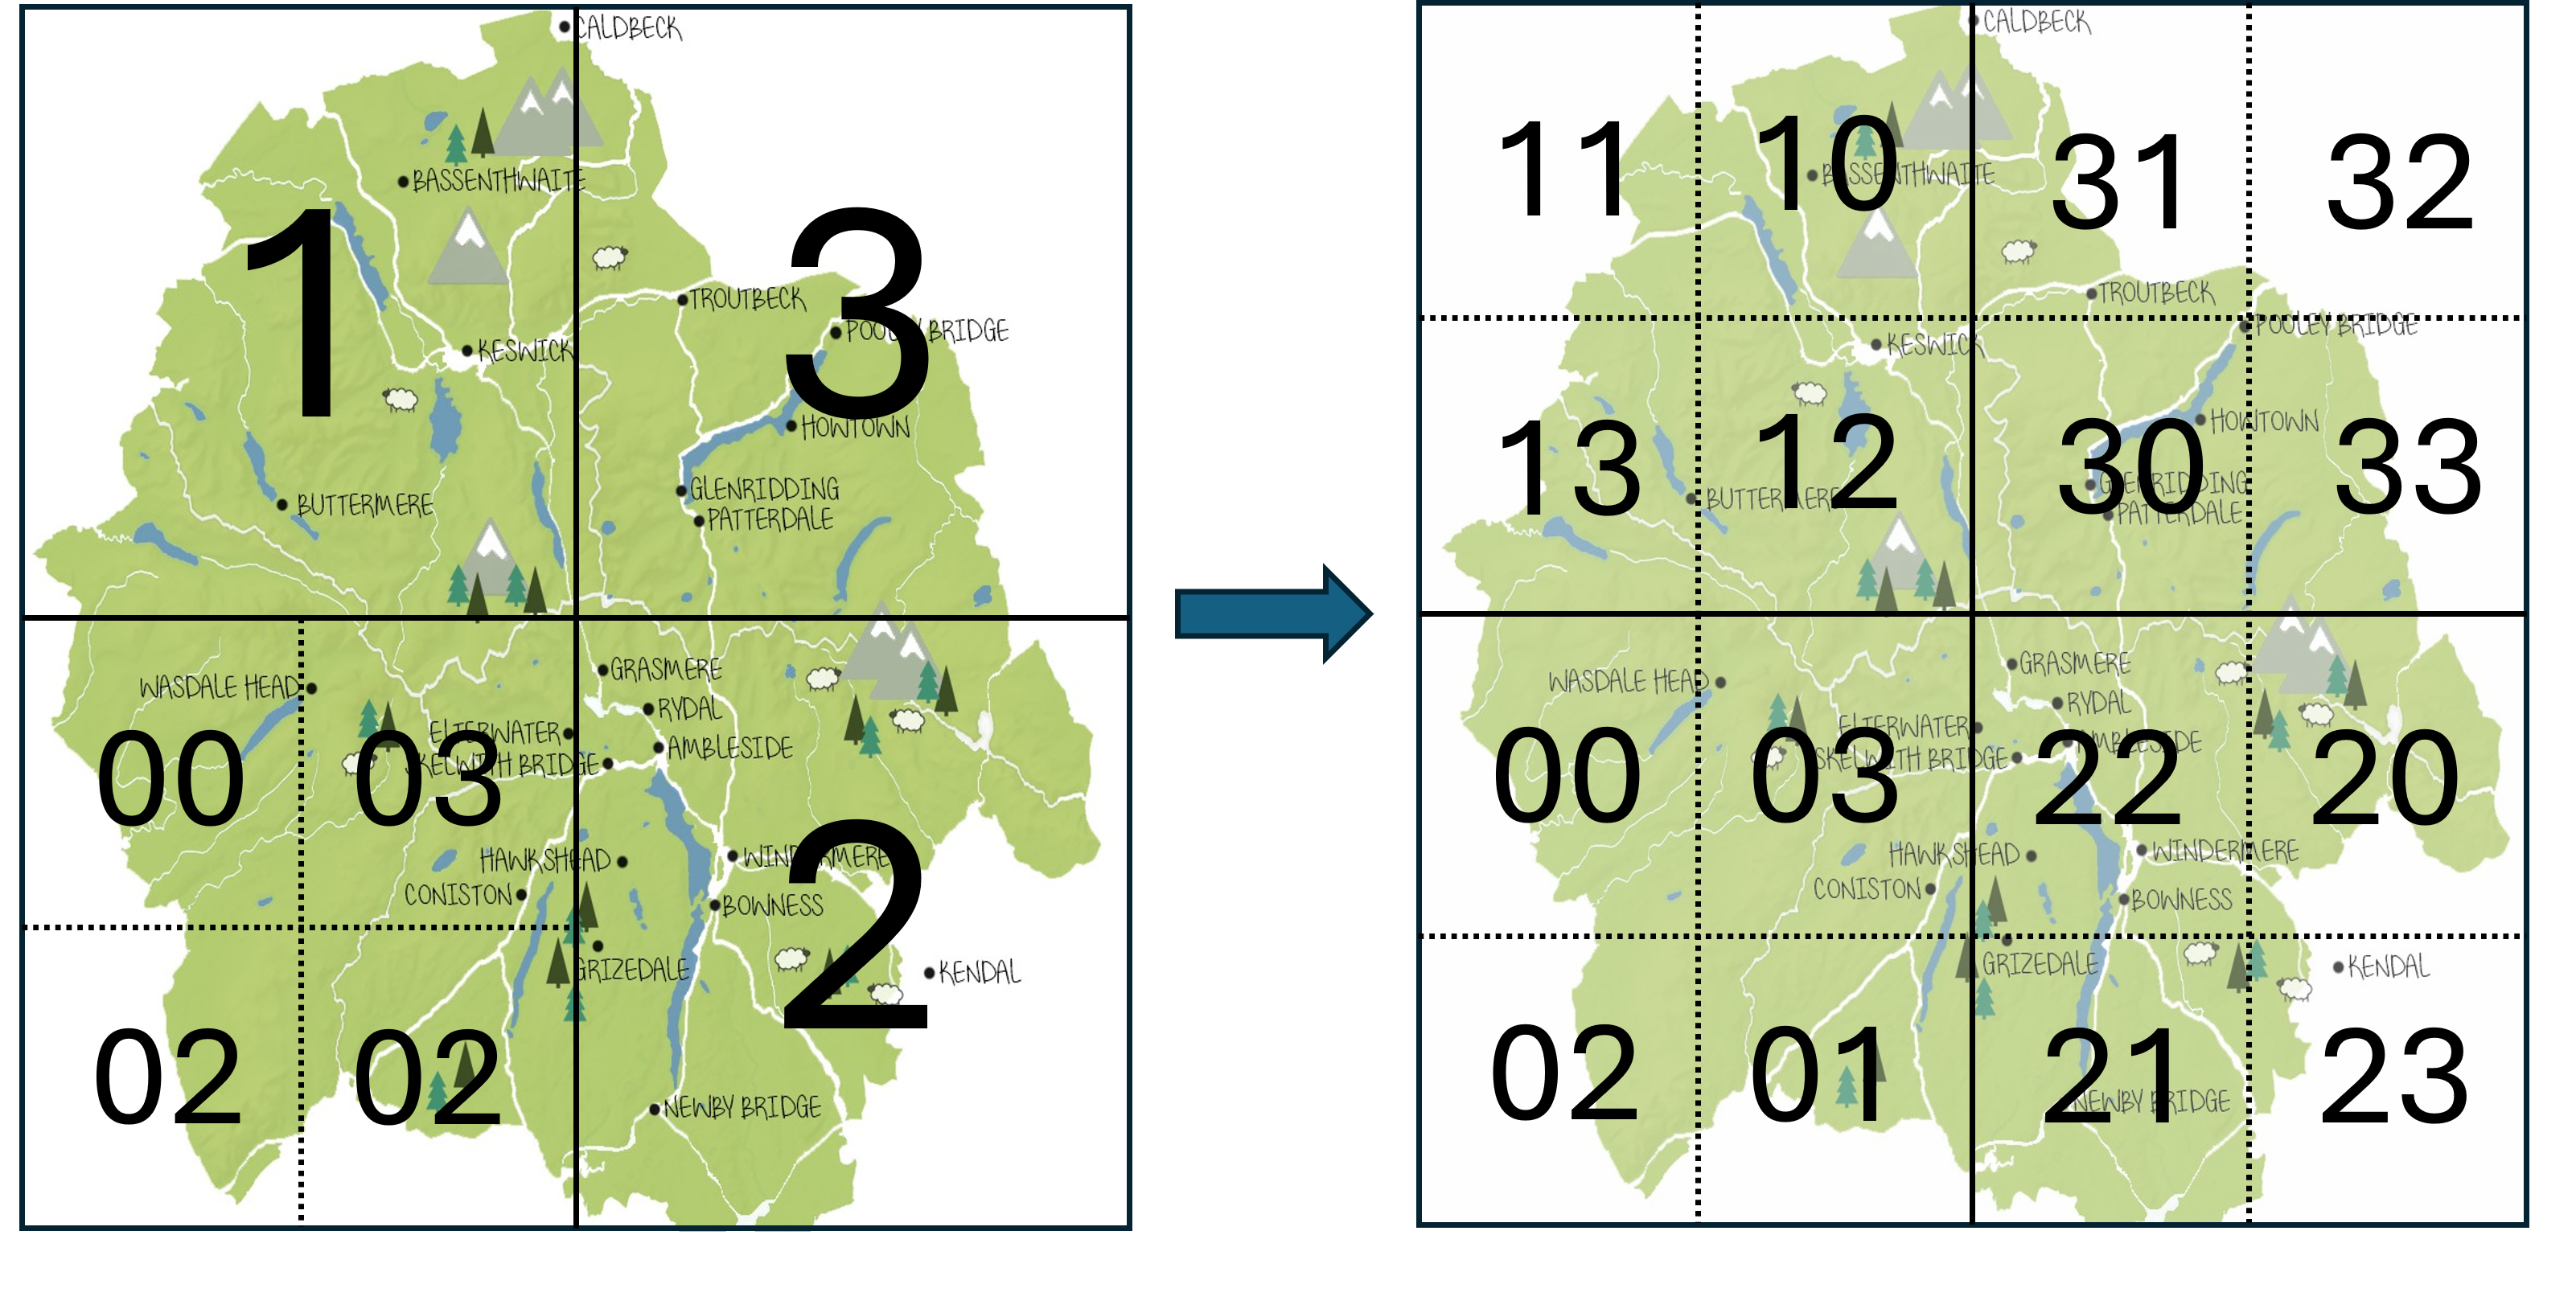
\includegraphics{images/lake_d3.png}
\end{center}

\begin{enumerate}
\def\labelenumi{\arabic{enumi}.}
\setcounter{enumi}{3}
\tightlist
\item
  Continue this hierarchical randomisation to the desired spatial scale
  such that
  \(\mathcal{A}_k \equiv \{a_1,\ldots,a_k:a_1 = 0,1,2,3; \ldots; a_k = 0,1,2,3\}\)
  until the sum of the inclusion probabilities of each element within a
  given square are less than one.
\end{enumerate}

\begin{center}
\includegraphics[width=3.125in,height=\textheight]{images/lake_d4.png}
\end{center}

\begin{enumerate}
\def\labelenumi{\arabic{enumi}.}
\setcounter{enumi}{4}
\tightlist
\item
  The elements (e.g., lakes) in \(\mathcal{A}_k\) are placed in
  hierachichal order by sorting out \(\mathcal{A}_k\) by the level 1
  cells from smallest to largest, then by the level-two cells from
  smallest to largest, and so on. This will transform the level \(k\)
  grid cell to a \textbf{one-dimensional number} line. The length of
  each line-segment represents the inclusion probability for a given
  site (or lake in this example). Thus, the line's total length equals
  the sum of these inclusion probabilities (the sum should equal \(n\)
  since we do not allow the inclusion value within a cell to be greater
  than one). Here we have colored cells contianing larger lakes in red
  and small lakes in blue.
\end{enumerate}

\begin{center}
\includegraphics{images/lake_d5.png}
\end{center}

\begin{enumerate}
\def\labelenumi{\arabic{enumi}.}
\setcounter{enumi}{5}
\tightlist
\item
  Then, we can use \textbf{systematic} sampling along the line to select
  the lakes to survey. E.g., you can randomly draw \(u_1\) from an
  uniform {[}0,1{]} and place it on a line. Imagine we draw
  \(u_1 = 0.53\), then location of \(u_1\) on the line falls within some
  line segment that represents a site, which we denote \(s_1\) (in the
  example this is the lake in cell 010). We include this sites as our
  first site in the sample and then continue with the next \(j\) sites
  by setting \(u_j = u_{j-1} +1\) for \(j = 2,\ldots,n\).
\end{enumerate}

\begin{center}
\includegraphics{images/lake_systematic.png}
\end{center}

\begin{enumerate}
\def\labelenumi{\arabic{enumi}.}
\setcounter{enumi}{6}
\tightlist
\item
  Suppose we would like larger lakes to be twice as likely to be
  selected as small lakes. Thus, instead of given all lakes the same
  unit length we can give large lakes twice the unit length of small
  lakes.
\end{enumerate}

\begin{center}
\includegraphics{images/lake_systematic_unequall.png}
\end{center}

In addition to unequal inclusion probabilities we can also perform
stratified sampling. Thus, instead of sampling from the entire sampling
frame simultaneously, we divide a sampling frame into distinct sets of
sites and select samples from each stratum independently of other strata
-we apply the GRTS algorithm to obtain stratum-specific sample sizes.
The R-package \texttt{spsurvey} implements GRTS algorithm to select
spatially balanced samples via the \texttt{grts()} function.

\subsection{Before-after-Impact
approaches}\label{before-after-impact-approaches}

The purpose of monitoring is to assess the changes in a particular
variable over time. This can typically be carried out using standard
statistical techniques, taking into account the structure of the data.
Sometimes we are interested in whether a specific event has had an
impact on the variable, e.g., the effect of new regulations on the air
pollution level. Typically this involves assessing the levels before and
after the event.

It is generally very difficult to untangle the effects of a single
event. Even if we identify a change in the mean or variance, how do we
know that it is due to our event? Many environmental systems change
naturally over time for any number of reasons. We do not have a
statistical control, meaning that we can't turn back the clock and check
what would have happened without the event.

However, this challenge is not unique to environmental data. We face it
regularly in statistics. Often, we are only interested in the effect of
one particular variable, but we have to account for other nuisance
variables via regression or other techniques. We can also sometimes
account for other unmeasured variability through random effects. The key
is to acknowledge what you do and don't know, and to account properly
for uncertainty.

\begin{tcolorbox}[enhanced jigsaw, arc=.35mm, colframe=quarto-callout-important-color-frame, breakable, colback=white, opacityback=0, colbacktitle=quarto-callout-important-color!10!white, toptitle=1mm, toprule=.15mm, coltitle=black, title={Examples: Before-After Designs}, left=2mm, rightrule=.15mm, bottomrule=.15mm, titlerule=0mm, bottomtitle=1mm, opacitybacktitle=0.6, leftrule=.75mm]

\begin{enumerate}
\def\labelenumi{\arabic{enumi}.}
\tightlist
\item
  \textbf{Before-After Single Site}
\end{enumerate}

Often, we wish to assess the impact of an intervention on a site, but we
only have data for that site.

\begin{figure}[H]

{\centering \includegraphics[width=3.125in,height=\textheight]{images/BASS.png}

}

\caption{Line graph of value by time, illustrating the impact of an
intervention. The blue arrows represent the time ``before'' the
intervation and the red arrows represent the time ``after'' the
intervantion.}

\end{figure}%

We can fit a statistical model, such as:
\[X_{ik} = \mu + \alpha_i + \tau_{k(i)} + \varepsilon_{ik}\] with
\(\mu\) representing the overall mean, \(\alpha_i\) the effect of period
(before/after), \(\tau_{k(i)}\) the time within period, and
\(\varepsilon_{ik}\) the errors.

This is not an ideal design, since we have no control to compare to.

\begin{enumerate}
\def\labelenumi{\arabic{enumi}.}
\setcounter{enumi}{1}
\tightlist
\item
  \textbf{Before-After Multiple Sites}
\end{enumerate}

We can sometimes improve upon the Before-After Single Site design, if we
can collect data at multiple \(j=1,\ldots,M\) sites that are likely to
be impacted by the intervention. We can fit a statistical model, such
as:

\[
X_{ijk} = \mu + \alpha_i + \tau_{jk(i)} + \delta_j + \varepsilon_{ijk},
\]

where \(\mu\) is the overall mean; \(\alpha_i\) is the effect of period
(before/after); \(\tau_{jk(i)}\) represents the time within the
\emph{i}th period; \(\delta_j\) is the site \(j\) random effect and
\(\varepsilon_{ijk}\) are the sampling errors.

\begin{figure}[H]

{\centering \includegraphics[width=3.125in,height=\textheight]{images/BAMS.png}

}

\caption{Line graph of value by time, illustrating the impact of an
intervention. Each line connects the data points for a single site.}

\end{figure}%

Treating the sites as \emph{subsamples} allows the sites to be used to
improve estimation of the effect's magnitude, compared to a single site
design.

\begin{enumerate}
\def\labelenumi{\arabic{enumi}.}
\setcounter{enumi}{2}
\tightlist
\item
  \textbf{Before-After Control-Impact (BACI)}
\end{enumerate}

BACI is a common design, where one or more potentially impacted sites,
and one or more sites that are thought not vulnerable to impact, are
sampled before and after the time of the intervention.

\begin{figure}[H]

{\centering \includegraphics[width=3.125in,height=\textheight]{images/BACI.png}

}

\caption{Line graph of value by time, illustrating the impact of an
intervention on the ``impact'' site. The two lines connect the data
points for two sites (one impact site and one control site).}

\end{figure}%

We can fit a statistical model, such as:
\[X_{ij} = \mu + \alpha_i + \beta_j + (\alpha\beta)_{ij} + \varepsilon_{ij}\]
with \(\mu\) representing the overall mean, \(\alpha_i\) the effect of
period (before/after), \(\beta_j\) the effect of location
(control/impact), and \(\varepsilon_{ik}\) the errors.

Having the control sites allows us to better assess whether any impacts
are \emph{caused by} the intervention.

\end{tcolorbox}

\phantomsection\label{refs}
\begin{CSLReferences}{1}{0}
\bibitem[\citeproctext]{ref-stevens2004}
Stevens, Don L, and Anthony R Olsen. 2004. {``Spatially Balanced
Sampling of Natural Resources.''} \emph{Journal of the American
Statistical Association} 99 (465): 262--78.
\url{https://doi.org/10.1198/016214504000000250}.

\end{CSLReferences}



\end{document}
